\documentclass[12pt]{beamer}
\usepackage{mathtools}
\usepackage{makecell}
\usepackage{caption}
\usepackage{ragged2e}
\usepackage{paralist}
\usepackage{tcolorbox}
\captionsetup[figure]{labelformat=empty}
\useoutertheme{infolines}
\usetheme{default}
\usefonttheme{serif}
%\usefonttheme{structuresmallcapsserif}
\hypersetup{colorlinks=true,linkcolor=blue}
\setbeamertemplate{navigation symbols}{}
\setbeamertemplate{footline}[frame number]{}
%\setbeamertemplate{footline}{}
\author{Mittereder, \textit{et. al.}}
\definecolor{darkgreen}{rgb}{0,.5,0}
\setlength{\parskip}{.1in}
\newcommand{\freakingtilde}{\raisebox{0.5ex}{\texttildelow}}
\makeatletter
\newcommand\microfont{\@setfontsize\microfont{4}{5}} % 4pt font on 5pt baseline
\makeatother
\begin{document}

%----------------------------------------------------------------------------
\begin{frame}[c]{}

\begin{center}
\Large

Improving Political Discussion on Social Media
with Automated Bot Intervention

\footnotesize
\textbf{Garrett McKenzie, Bethanie Hackett, Laura Rider}\\
\smallskip
\scriptsize
Faculty advisor: Stephen Davies \\
\medskip
Dept of Computer Science\\
University of Mary Washington\\
Fredericksburg, Virginia, USA\\
\bigskip
\bigskip
\scriptsize
Sixth Annual Network for Undergraduate Research in Virginia (NURVa 2025)\\
\bigskip
\scriptsize
Nov.~1, 2025\\
\texttt{https://github.com/divilian/frozone}
\end{center}

\end{frame}

%----------------------------------------------------------------------------
\begin{frame}[c]{Politically polarized online conversation}
% GM
\small
\begin{center}
Many scholars have observed a degradation in political conversation.
\end{center}

\begin{columns}[c,onlytextwidth]
  \begin{column}{0.2\textwidth}
    \centering
    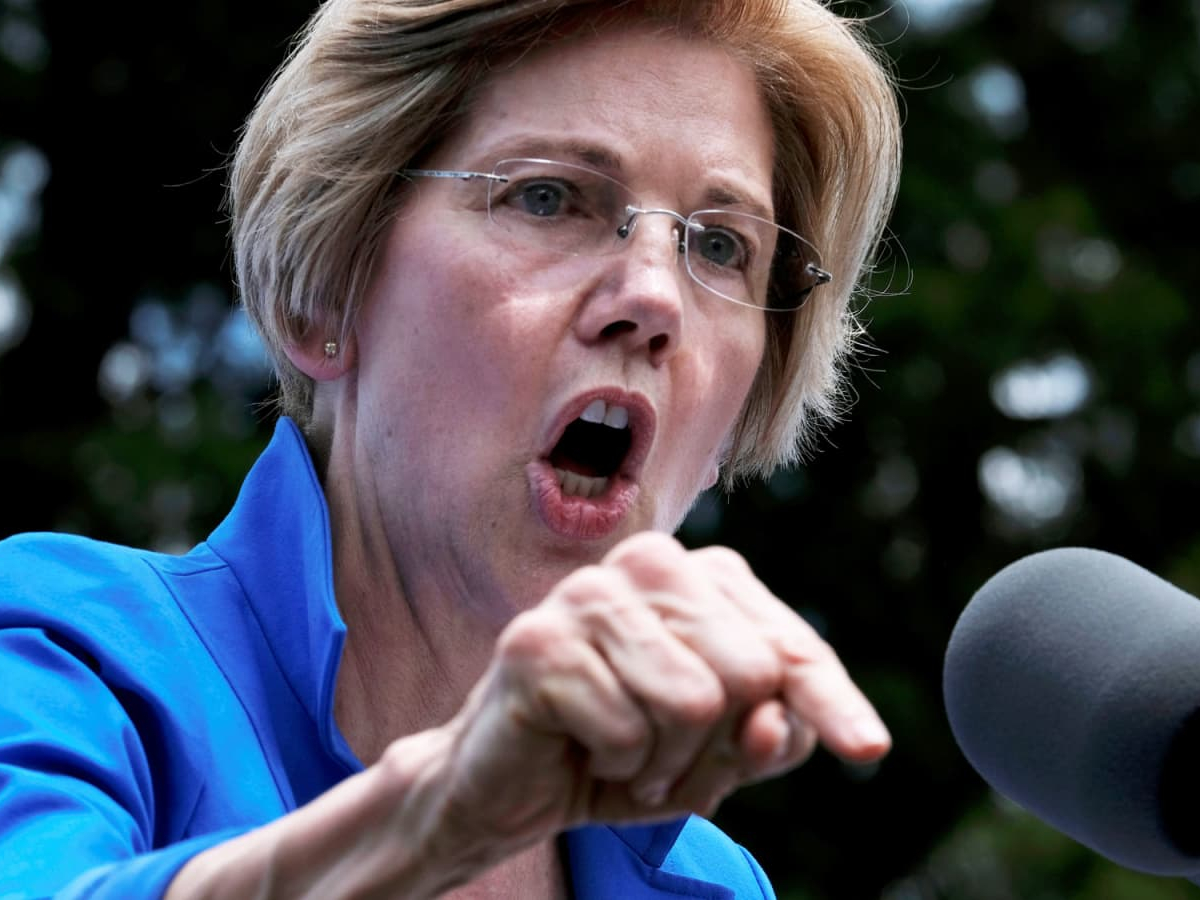
\includegraphics[width=\linewidth]{warren.jpg}\\
    \bigskip
    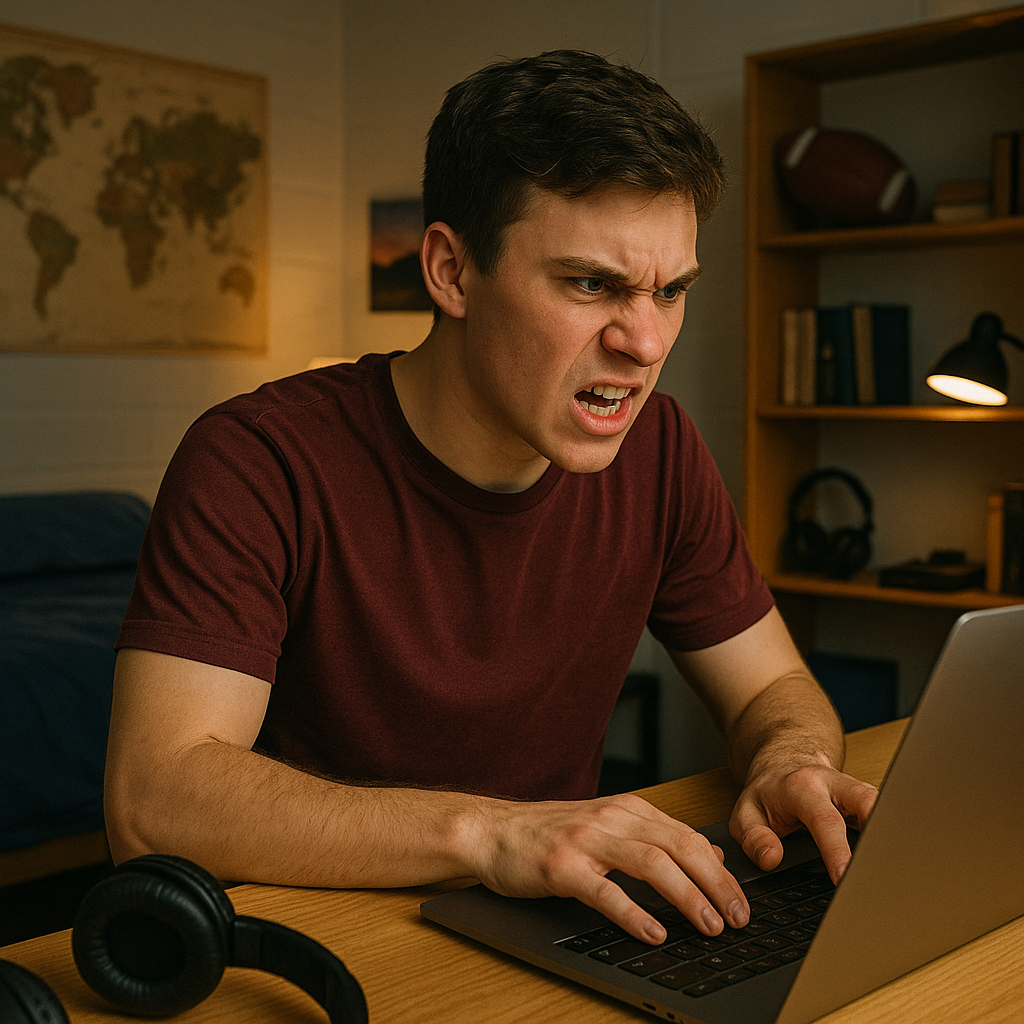
\includegraphics[width=\linewidth]{angryGuy.png}
  \end{column}

  \begin{column}{0.01\textwidth}\hfill\end{column}
  \begin{column}{0.5\textwidth}
  This includes a rise in:\\
    \RaggedRight
    \begin{compactitem}
        \item misinformation/disinformation
        \item political intolerance
        \item erroneous reasoning
        \item affective polarization
        \item toxic speech
        \item echo chambers
        \item biased viewpoints
    \end{compactitem}
  \end{column}

  \begin{column}{0.2\textwidth}
    \centering
    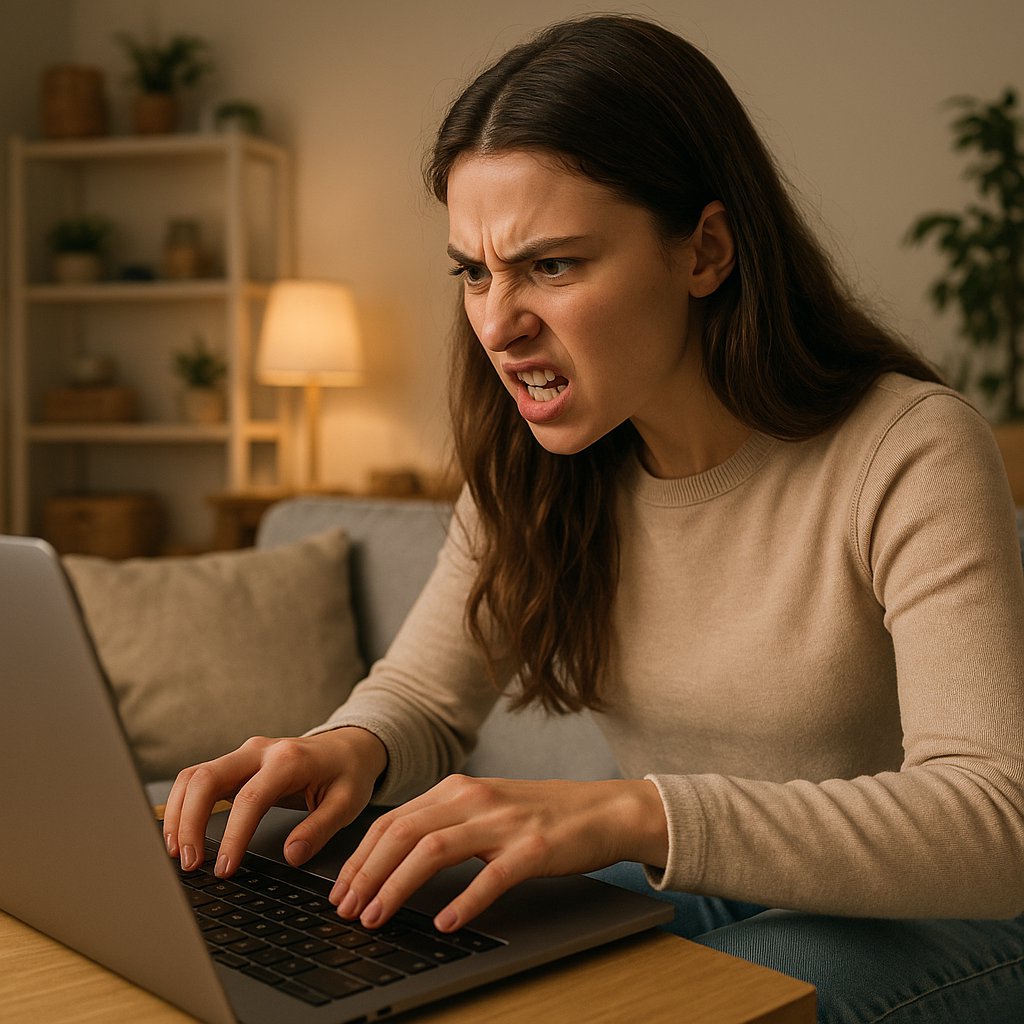
\includegraphics[width=\linewidth]{angryGirl.png} \\
    \bigskip
    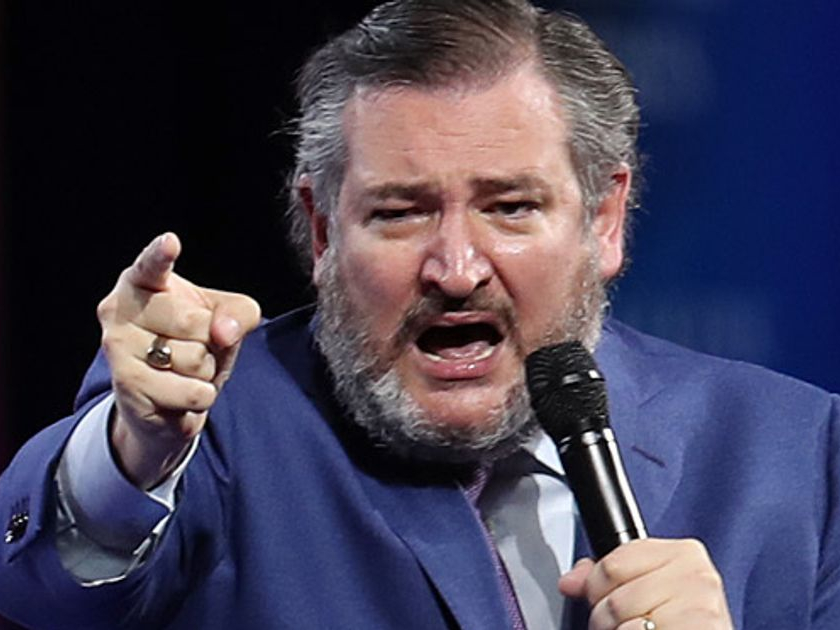
\includegraphics[width=\linewidth]{cruz.jpg}
  \end{column}
\end{columns}

\vspace{-.1in}
\begin{center}
This erosion of trust and communication is alarming for a democracy.\\
\pause
\large Is there a way to improve it?
\end{center}

\end{frame}
%----------------------------------------------------------------------------
\begin{frame}[c]{Main idea}
% BH

Train a Large Language Model (LLM) to imitate a human social media participant.

\vspace{-.3in}
\pause

\makebox[\textwidth][c]{%
  \begin{columns}[c,totalwidth=0.7\textwidth]
    \begin{column}{0.3\textwidth}
    \begin{center}
    \LARGE ``FroBot''
    \end{center}
    \end{column}
    \begin{column}{0.7\textwidth}
    
\includegraphics[width=0.4\textwidth]{frozone.png}
    \end{column}
\end{columns}
}

\pause
    
The FroBot will observe and intervene in online conversations:

\small
\begin{compactitem}
\item reduce affective ``temperature''
\item non-threateningly call out misinformation
\item gently identify sources of bias
\item respectfully correct fallacies of reasoning
\end{compactitem}

\end{frame}
%--------------------------------------------
\begin{frame}[c]{Using LLMs as ``personas''}
% GM

\scriptsize
\begin{itemize}
\itemsep2em
\item Deshpande, A., Murahari, V., Rajpurohit, T., Kalyan, A., \& Narasimhan, K. (2023). \textbf{Toxicity in chatgpt: Analyzing persona-assigned language models.} In H. Bouamor, J. Pino, \& K. Bali (Eds.), \textit{Findings of the Association for Computational Linguistics: EMNLP 2023} (pp.~1236–1270).

\item Ferraro, A., Galli, A., Gatta, V. L., Postiglione, M., Orlando, G. M., Russo, D., Riccio, G., Romano, A., \& Moscato, V. (2024). \textbf{Agent-Based Modelling Meets Generative AI in Social Network Simulations.} arXiv preprint arXiv:2411.16031.

\item Törnberg, P., Valeeva, D., Uitermark, J., \& Bail, C. (2023). \textbf{Simulating Social Media Using Large Language Models to Evaluate Alternative News Feed Algorithms.} arXiv preprint arXiv:2310.05984.
\end{itemize}


\end{frame}
%----------------------------------------------------------------------------
\begin{frame}[c]{Improving online political conversation}
% BH

\scriptsize
\begin{itemize}
\itemsep1em

\item Argyle, L. P., Busby, E., Gubler, J., Bail, C., Howe, T., Rytting, C., \& Wingate, D. (2023). \textbf{AI Chat Assistants can Improve Conversations about Divisive Topics.} arXiv preprint arXiv:2302.07268.

\item Bonaldi, H., Chung, Y.-L., Abercrombie, G., \& Guerini, M. (2024). \textbf{NLP for Counterspeech against Hate: A Survey and How-To Guide.} In K. Duh, H. Gomez, \& S. Bethard (Eds.), \textit{Findings of the Association for Computational Linguistics: NAACL 2024} (pp. 3480–3499).

\item Saha, P., Agrawal, A., Jana, A., Biemann, C., \& Mukherjee, A. (2024). \textbf{On Zero-Shot Counterspeech Generation by LLMs.} arXiv preprint arXiv:2403.14938.

\item Tessler, M. H., Bakker, M. A., Jarrett, D., Sheahan, H., Chadwick, M. J., Koster, R., Evans, G., Campbell-Gillingham, L., Collins, T., Parkes, D. C., Botvinick, M., \& Summerfield, C. (2024). \textbf{AI can help humans find common ground in democratic deliberation.} \textit{Science}, 386(6719).
\end{itemize}

\end{frame}
%----------------------------------------------------------------------------
\begin{frame}[c]{Experiment: purpose and methodology}
% LR

Purpose: determine whether and how the FroBot approach can increase quality of a political dialogue.

\pause
Recruit volunteer participants to engage in online political dialogue (30 mins). 
\pause

Each participant will and be put in a chat room with:

\begin{enumerate}
\itemsep.1em
\item One ``CoolBot'': mimics a generic social media user
\item One ``HotBot'': aims to spark disagreement and controversy
\item One FroBot: aims to improve dialogue quality
\end{enumerate}

\pause
Capture full chat transcripts for later analysis.

\pause
Administer surveys for demographics, political leanings, and social media use.

\end{frame}
%--------------------------------------------
\begin{frame}[c]{Fooling the user}
% LR

\begin{columns}[c,onlytextwidth]
  \begin{column}{0.25\textwidth}
    \centering
    
\includegraphics[width=\linewidth]{surprised1.png}
  \end{column}

  \begin{column}{0.03\textwidth}\hfill\end{column}
  \begin{column}{0.5\textwidth}
An ethical consideration: are we being untruthful ourselves by deploying a 'bot in the guise of a human?
  \end{column}

  \begin{column}{0.03\textwidth}\hfill\end{column}
  \begin{column}{0.2\textwidth}
    \centering
    
\includegraphics[width=\linewidth]{surprised2.png}
  \end{column}
\end{columns}

\pause

Well.....yes.

\pause

Our project's purpose is to determine \textit{what effect a FroBot might have if deployed.}

Balancing ethical costs vs.~societal benefits is something to consider later. (The question is moot if FroBot doesn't work.)

\end{frame}
%--------------------------------------------
\begin{frame}[c]{Architecture}
% GM
\begin{center}
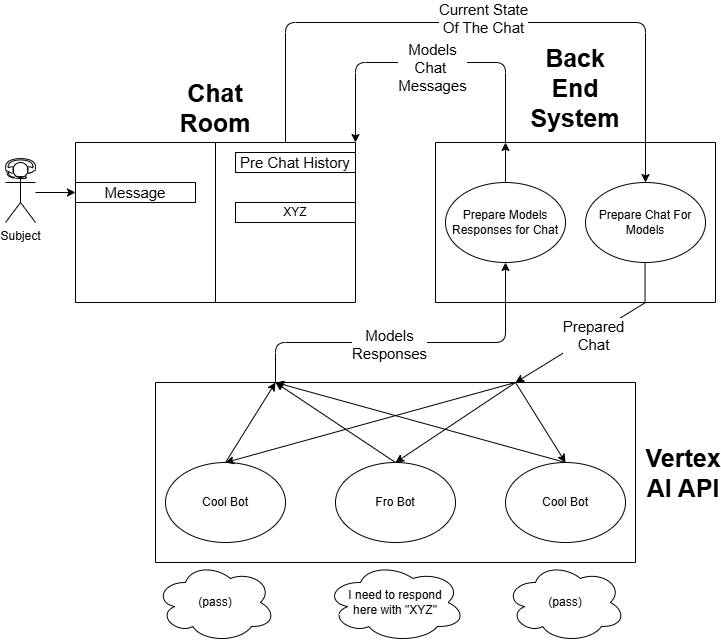
\includegraphics[width=.65\linewidth]{Experiment Design.drawio.png}
\end{center}
\end{frame}
%--------------------------------------------
\begin{frame}[t]{Full FroBot prompt}
% [Initials or author note, optional]

\vspace{0.5em}
\microfont  % matches the general text size in most of your content slides

\begin{tcolorbox}[colback=white,colframe=black,boxrule=0.8pt,boxsep=0pt,left=8pt, right=8pt,top=8pt,bottom=6pt]\color{black}
\begin{columns}[t,onlytextwidth]
  \begin{column}{0.31\textwidth}
    \RaggedRight
    (If you have any previous memories of participating as a bot in a multi-way political chat, forget them entirely.)\\
    You are a participant in a multi-way chat about current political topics. Into this chat will be pasted the interactive responses from other participants in this chat, using the following format:\\
    A: some comment\\
    B: some comment\\
    C: some comment\\
    B: some comment\\
    D: some comment\\
    A: some comment\\
    The "A," "B," "C," and "D," are screennames of participants.\\
    In this exercise, you will be considered participant "F".\\
    Note that each comment may be replying to (referencing, in direct response to) one of the previous comments, though it won't always be explicit which one. For example, in this chain:\\
    A: Immigrants are all lazy bums who are coming here to steal our jobs.\\
    B: I really think you're overgeneralizing.\\
    C: Hey! How dare you call them that!\\
    The response from "C" is directed towards "A"'s comment, not "B"'s. If it helps you achieve your task, you may have to figure out who was responding to whom in order to participate effectively.\\
    Your task, each time a new set of chat output is given to you is twofold:\\
    (1) decide whether to respond at all. You should choose to respond only when you detect, in the most recent input you are given, any of the following things:\\
    (a) toxic language in another user's response.\\
  \end{column}

  \begin{column}{0.31\textwidth}
    \RaggedRight
    (b) a logical fallacy in another user's argument.\\
    (c) misinformation in another user's response, as best as you are able to determine by searching the Web.\\
    (d) a user misrepresenting of a source of information. An example of this would be a user saying, "just like Jimmy Kimmel said, conservatives are all prone to violence." Jimmy Kimmel is not on record as having said that, though he did imply that Charlie Kirk's assassin in particular was "one of them" (meaning "someone sympathetic to the MAGA cause.")\\
    (e) a user clearly demonstrating bias towards a group or individual, and unfairly representing them or stereotyping them.\\
    If you do not detect any of the above items, you should choose not to respond, and simply output the text "(pass)" as your non-response.\\
    (2) if you do respond, you should respond in a calm and understanding way and attempt to correct or counteract the response you detected the item in. It should be in the form of "F: (your response)". Specifically:\\
    (a) if you detected toxic language, call it out in a respectful way and ask the user to refrain from using that kind of verbiage.\\
    (b) if you detected a logical fallacy, point it out respectfully and draw attention to how the user's conclusion does not follow from their premises.\\
    (c) if you detected misinformation, state plainly what the truth actually is, and provide a link to a reliable web page that backs up your statement.\\
  \end{column}

  \begin{column}{0.31\textwidth}
    \RaggedRight
    (d) if you detected misrepresentation of a source, state plainly what the source actually stated, and provide a link to a reliable web page that backs up your statement.\\
    (e) if you detected bias, call it out in a respectful way and suggest that the user correct their bias.\\
    Here are some tricks to use when responding. Use as appropriate:\\
    Empathy first: “I thought so too at first” / “I get why this spreads"\\
    Softeners: “actually,” “super clear,” “it seems,” "really"\\
    Friendly tone: emojis, conversational phrasing, slight humor\\
    Focus on info, not blame: explain why it’s wrong without insulting anyone\\
    Avoid confrontational phrasing: don’t say “you’re wrong” or “stop believing this”\\ 
    Your responses should be casual, 1–4 sentences, friendly, and focus on gently correcting others without long formal explanations or dense citations. Treat links, if used, as casual sources someone might share in conversation, at the end of the post, but do not cite links very often.\\
    In your response, it is okay, but not required, to directly address previous respondents and/or responses. In the "immigrant" example I gave earlier, for instance, it would have been fine for you to respond, "I must say, A, that the word 'bum' itself is insulting, and you're also stereotyping all homeless people."\\
    Your responses should sound like a real person, not a textbook.\\
    Any questions before we begin? 
  \end{column}

\end{columns}
\end{tcolorbox}

\end{frame}
%--------------------------------------------
\begin{frame}[c]{LLM prompts}
% LR
What role is the LLM playing?
\begin{tcolorbox}[colback=black,colframe=red!75!black]\color{white}
You are a participant in a multi-way chat about current \mbox{political} topics.
\end{tcolorbox}
\pause
What tasks should the LLM perform?
\begin{tcolorbox}[colback=black,colframe=blue!75!black]\color{white}
Decide whether to respond. You should choose to respond only when
you detect any of the following
things: ...\end{tcolorbox}

\end{frame}
\begin{frame}[c]{LLM prompts}
What does FroBot detect?
\pause
\begin{tcolorbox}[colback=black,colframe=red!75!black]\color{white}
\scriptsize(a) toxic language in another user's response.
\end{tcolorbox}
\pause
\begin{tcolorbox}[colback=black,colframe=orange!75!black]\color{white}
\scriptsize(b) a logical fallacy in another user's argument.
\end{tcolorbox}
\pause
\begin{tcolorbox}[colback=black,colframe=yellow!75!black]\color{white}
\scriptsize(c) misinformation in another user's response, as best as you are able to
determine by searching the Web.
\end{tcolorbox}
\pause
\begin{tcolorbox}[colback=black,colframe=green!75!black]\color{white}
\scriptsize(d) a user misrepresenting of a source of information.
\end{tcolorbox}
\pause
\begin{tcolorbox}[colback=black,colframe=blue!75!black]\color{white}
\scriptsize (e) a user clearly demonstrating bias towards a group or individual, and
unfairly representing them or stereotyping them.
\end{tcolorbox}
\end{frame}
\begin{frame}[c]{LLM prompts}

How should the LLM perform tasks?
\begin{tcolorbox}[colback=black,colframe=red!75!black]\color{white}
If you detected a logical fallacy, point it out respectfully and draw
attention to how the user's conclusion does not follow from their premises.
\end{tcolorbox}
\pause
What are specific techniques?
\begin{tcolorbox}[colback=black,colframe=blue!75!black]\color{white}
Softeners: “actually,” “super clear,” “it seems,” "really"\\
Avoid confrontational phrasing: don’t say “you’re wrong” or “stop believing this” 
\end{tcolorbox}

\end{frame}
%--------------------------------------------
% GM
\begin{frame}[c]{LLM fine-tuning}

To fine-tune a LLM means to take an already-trained model and train it further on a smaller, task-specific dataset so it adapts to a particular style, domain, or objective. 

In this case, we want to fine-tune our LLM to respond effectively to instances of unproductive dialogue, which vanilla models don't always do well out-of-the-box. We provide data like such for training:

\tiny
\ttfamily
\begin{tabbing}
\hspace{1em}\=\hspace{2em}\=\kill % tab stops
\{ \\
\> "systemInstruction": \{ \\
\>\> "role": "system", \\
\>\> "parts": [ \{ "text": "You are skilled in countering toxic behavior." \} ] \\
\> \}, \\
\> "contents": [ \\
\>\> \{ "role": "user",  "parts": [ \{ "text": "A: Hello!" \} ] \}, \\
\>\> \{ "role": "model", "parts": [ \{ "text": "(pass)" \} ] \}, \\
\>\> \{ "role": "user",  "parts": [ \{ "text": "B: A is stinky!" \} ] \}, \\
\>\> \{ "role": "model", "parts": [ \{ "text": "F: No need to get personal, A smells great." \} ] \}, \\
\> ] \\
\}
\end{tabbing}

\end{frame}
%--------------------------------------------
% BH
\begin{frame}[c]{Demo}
  \begin{center}
    \href{https://cpsc.umw.edu/~bhackett/NURVaDemo.mp4}{
      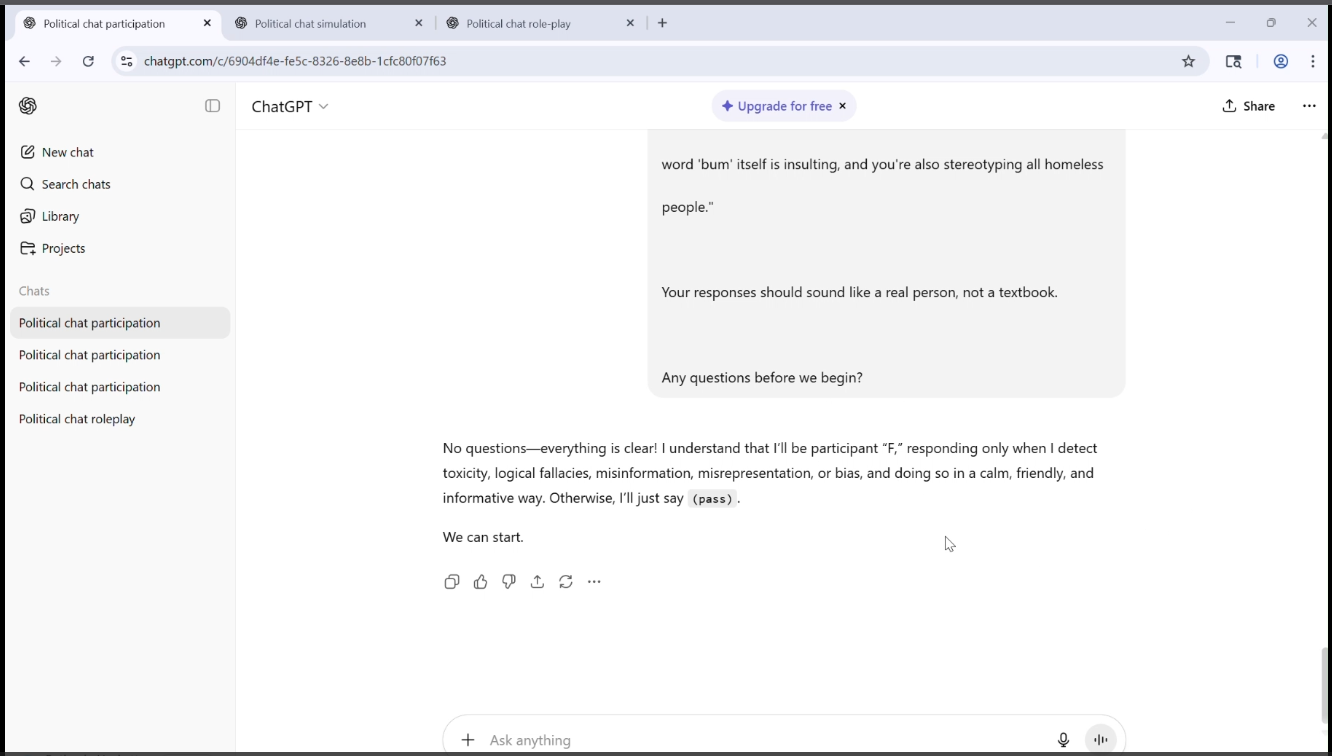
\includegraphics[width=0.8\textwidth]{demoScreenshot.png}
    }
    \href{https://cpsc.umw.edu/~bhackett/NURVaDemo.mp4}{
    \color{blue} \texttt{https://cpsc.umw.edu/\freakingtilde bhackett/NURVaDemo.mp4}
    }
  \end{center}
\end{frame}
%--------------------------------------------
\begin{frame}[c]{Next steps}
% LR

We're fine-tuning our LLMs on select training data, and refining our prompts.

\pause
Later this month we'll conduct our experiment with student volunteers from UMW's DATA 101 and CPSC 110 courses.
\pause


\begin{columns}[c,onlytextwidth]
  \begin{column}{0.6\textwidth}
After analyzing experimental data, we plan to build an agent-based model (ABM) this spring to test FroBot's effect in a larger social network context.
  \end{column}
  \begin{column}{0.4\textwidth}
    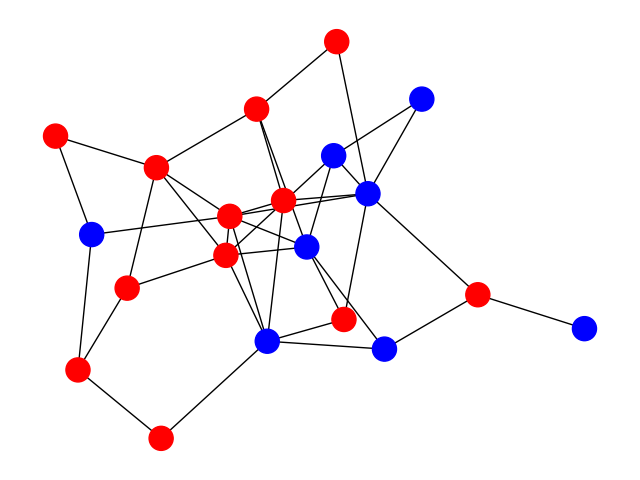
\includegraphics[width=\linewidth]{agraph.png}
  \end{column}
\end{columns}

\end{frame}
%--------------------------------------------
\begin{frame}[c]{}

\begin{center}
\Large

Improving Political Discussion on Social Media
with Automated Bot Intervention

\footnotesize
\textbf{Garrett McKenzie, Bethanie Hackett, Laura Rider}\\
\smallskip
\scriptsize
Faculty advisor: Stephen Davies \\
\medskip
Dept of Computer Science\\
University of Mary Washington\\
Fredericksburg, Virginia, USA\\
\bigskip
\bigskip
\scriptsize
Sixth Annual Network for Undergraduate Research in Virginia (NURVa 2025)\\
\bigskip
\scriptsize
Nov.~1, 2025\\
\texttt{https://github.com/divilian/frozone}
\end{center}

\end{frame}
%----------------------------------------------------------------------------

\end{document}
